\documentclass[../../main.tex]{subfiles}

\begin{document}

\subsection{Unità di misura-grandezze fondamentali}
\begin{enumerate}
    \item \textbf{Lunghezza (m)}: Misura l'estensione di un oggetto in una direzione specifica.
    \item \textbf{Massa (kg)}: Misura la quantità di materia in un corpo.
    \item \textbf{Tempo (s)}: Misura la durata di un evento o intervallo tra due istanti.
    \item \textbf{Densità ($\frac{kg}{m^3}$)}: Misura la quantità di massa contenuta in un certo volume.
    \item \textbf{Corrente elettrica (A)}: Misura la quantità di carica elettrica che fluisce attraverso un circuito in un certo tempo.
\end{enumerate}
Il sistema che ha definito le precedenti unità di misura come fondamentali è il \textbf{Sistema Internazionale (SI) (MKSA)}.
\subsection{Velocità}
\[
    \text{Velocità} = \frac{\text{spazio percorso}}{\text{tempo impiegato}}
\]
L'unità di misura della velocità è il $\frac{m}{s}$ ed è detta unità di misura derivata in quanto è ottenuta da unità di misura fondamentali.\\
La fisica è fatta di misurazioni, ma le misurazioni comportano errori e quindi è necessario definire la precisione di una misurazione.\\
\subsection{Notazione scientifica}
Fondamentale per esprimere numeri molto grandi o molto piccoli.
\subsection{Multipli e sottomultipli}
\begin{itemize}
    \item $10^15$ = Peta (P)
    \item $10^12$ = Tera (T)
    \item $10^9$ = Giga (G)
    \item $10^6$ = Mega (M)
    \item $10^3$ = Kilo (K)
    \item $10^{-3}$ = Milli (m)
    \item $10^{-6}$ = Micro ($\mu$)
    \item $10^{-9}$ = Nano (n)
    \item $10^{-12}$ = Pico (p)
    \item $10^{-15}$ = Femto (f)
    \item $10^{-18}$ = Atto (a)
\end{itemize}
\newpage
\subsection{Grandezze fisiche}
\begin{table}[h!]
    \centering
    \begin{tabular}{|c|c|c|c|c|}
        \hline
        \textbf{Grandezza}     & \textbf{Simbolo} & \textbf{Unità di misura} & \textbf{Dimensioni}        & \textbf{Unità SI}           \\
        \hline
        Velocità               & $\bar v$         & $\frac{m}{s}$            & $L \cdot T^{-1}$           & $m \cdot s^{-1}$            \\
        Accelerazione          & $\bar a$         & $\frac{m}{s^2}$          & $L \cdot T^{-2}$           & $m \cdot s^{-2}$            \\
        Accelerazione angolare & $\alpha$         & $\frac{rad}{s^2}$        & $T^{-2}$                   & $rad \cdot s^{-2}$          \\
        Densità                & $\rho$           & $\frac{kg}{m^3}$         & $M \cdot L^{-3}$           & $kg \cdot m^{-3}$           \\
        Lunghezza              & $L$              & $m$                      & $L$                        & $m$                         \\
        Massa                  & $m$              & $kg$                     & $M$                        & $kg$                        \\
        Tempo                  & $t$              & $s$                      & $T$                        & $s$                         \\
        Energia                & $E, \ U, \ K$    & $J$                      & $\dfrac{M \cdot L^2}{T^2}$ & $kg \cdot m^2 \cdot s^{-2}$ \\
        Frequenza              & $f$              & $Hz$                     & $T^{-1}$                   & $s^{-1}$                    \\
        Forza                  & $\bar{F}$        & $N$                      & $M \cdot L \cdot T^{-2}$   & $kg \cdot m \cdot s^{-2}$   \\
        Volume                 & $V$              & $m^3$                    & $L^3$                      & $m^3$                       \\
        \hline
    \end{tabular}
\end{table}
\subsection{Angolo}
\begin{figure}[h!]
    \begin{minipage}{0.45\linewidth}
        \begin{tikzpicture}
            \draw (0,0) circle (3cm);
            \draw[->] (0,0) -- (3,0) node[right] {$x$};
            \draw[->] (0,0) -- (0,3) node[above] {$y$};
            \draw[->] (0,0) -- (2.1,2.1) node[above] {$\vec{r}$};
            \draw (0.5,0) arc (0:45:0.5) node[midway, right] {$\theta$};
        \end{tikzpicture}
    \end{minipage}
    \hfill
    \begin{minipage}{0.5\linewidth}
        Gli angoli non hanno dimensioni, si misurano in radianti.
        \[
            \theta = \frac{L}{R} \implies \dfrac{\text{\sout{m}}}{\text{\sout{m}}} \implies \text{Radianti}
        \]
    \end{minipage}
\end{figure}
\subsection{Densità di massa}
La densità è il rapporto tra la massa e il volume.
\[
    \rho = \frac{m}{V}
\]
Per definizione la densità dell'acqua è $1 \frac{g}{cm^3} = 1000 \frac{kg}{m^3}$.\\
\subsubsection{Esercizio}
Quale è la massa in chilogrammi di due litri di elio, dove $1.00l = 1.00 \cdot 10^3 cm^3$ e la densità dell'elio è $0.1785 \frac{kg}{m^3}$?\\
\[
    \rho = \frac{m}{V} \implies m = \rho \cdot V \implies m = 0.1785 \frac{kg}{m^3} \cdot 2 \cdot 10^{3} cm^3 \implies 10^{-6} m^3 = 3.57 \cdot 10^{-4} kg
\]

\newpage
\section{Moto}
Il moto è il movimento dei corpi.
\subsection{Moto Rettilineo}
Il moto più semplice è il moto rettilineo, ovvero il moto lungo una retta. Inizialmente studiamo il moto di un corpo puntiforme.
Quando si parla di moto dobbiamo definire un'origine degli spazi e orientare la retta, in modo da determinare il verso positivo e
negativo.\\
Effettuando delle misurazioni si ottiene un diagramma orario e successivamente si può ottenere il grafico spazio-tempo.\\
\begin{figure}[h!]
    \centering
    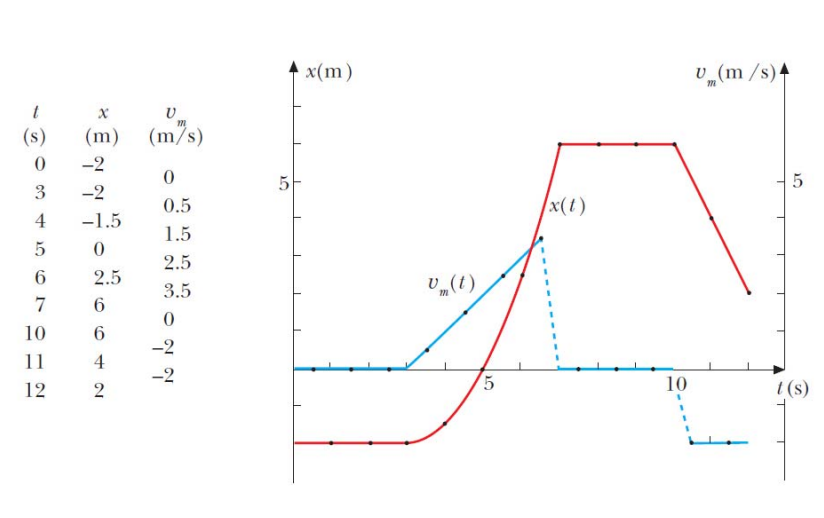
\includegraphics[width=0.6\textwidth]{Screenshot 2024-02-19 132549.png}
    \caption{Grafico spazio-tempo}
\end{figure}
\subsubsection{Velocità media}
\[
    \textbf{$\bar{v}_m$} = \frac{\Delta x}{\Delta t} = \frac{x_F - x_I}{t_F - t_I}
\]
\subsubsection{Velocità istantanea}
La velocità istantanea è una variazione piccolissima variazione di spazio in un piccolissimo intervallo di tempo.
\[
    \textbf{v} = \lim_{\Delta t \to 0} \frac{\Delta x}{\Delta t} = \frac{dx}{dt}
\]

\subsubsection{Due punti in moto sullo stesso asse}
Due punti materiali si trovano nell’istante iniziale $t = 0$ sullo stesso asse $x$, rispettivamente nella posizione $x_1$ con
velocità $v_1$ e nella posizione $x_2 > x_1$ con velocità $v_2$. Il moto dei punti è uniforme. Discutere quali sono le situazioni in
cui i punti ad un certo istante si urtano e determinare dove e quando si urtano.\\
Moto rettilineo uniforme $\iff$ velocità costante.\\
\[
    v = \frac{dx}{dt} \implies dx = v \cdot dt \implies \int_{0}^{t_0} dx = \int_{0}^{t_0} v(t) \cdot dt
\]
\[
    x(t_0) - x(0) = \int_{0}^{t_0} v(t) \cdot dt \implies x(t_0) - x(0) = \int_{0}^{t_0} v \cdot dt \implies x(t_0) - x(0) = v_0(t_0 - 0) \implies x(t_0) = v_0 \cdot t_0
\]
\[
    x_1(t) = v_1 \cdot t \quad x_2(t) = v_2 \cdot t + x_2(0)
\]
\begin{figure}
    \centering
    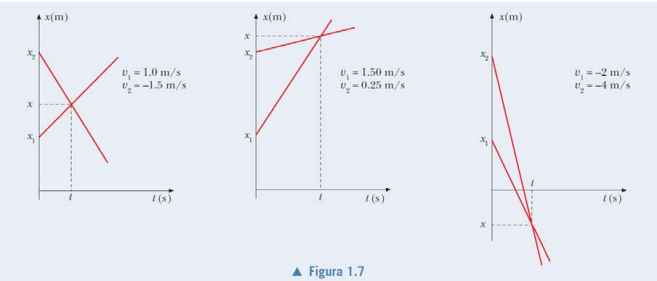
\includegraphics[width=0.8\textwidth]{9a2591ca-93e4-42c3-a861-5f067fd67bdb.png}
    \caption{Esempi di grafici di due punti in moto sullo stesso asse}
\end{figure}

\subsection{Accelerazione nel moto rettilineo}
Si definisce accelerazione e si indica con $\bar a$ il rapporto tra la velocità in un certo istante e l'intervallo di tempo in cui si è verificata la variazione di velocità.
\[
    a_m = \frac{\Delta v}{\Delta t} = \frac{v_2 - v_1}{t_2 - t_1}
\]
\[
    a_i = \lim_{\Delta t \to 0} \frac{\Delta v}{\Delta t} = \frac{dv}{dt} \implies v = \frac{dx}{dt} \implies a = \frac{d^2x}{dt^2}
\]
Anche quando la velocità diminuisce si ha un'accelerazione, ma negativa.\\
Se conosco l'accelerazione posso calcolare la velocità.
\[
    \dfrac{dv}{dt} = a \implies \int_{v_0}^{v_1} dv = \int_{0}^{t_1} a \cdot dt \implies v_1 - v_0 = \int_{t_0}^{t_1} a(t) \cdot dt
\]
\[
    v(t) = v(t_0) + \int_{t_0}^{t} a(t) \cdot dt
\]
\subsection{Moto rettilineo uniformemente accelerato}
Moto rettilineo uniformemente accelerato $\iff$ accelerazione costante.\\
\[
    dv = a dt \implies \int_{v_0}^v dv = \int_{0}^t a dt \implies v - v_0 = a \int_{0}^t dt = a \cdot t \implies v = v_0 + a \cdot t
\]
\[
    v = \dfrac{dx}{dt} \implies dx = v \cdot dt \implies dx = [v_0 + a(t - t_0)]dt \implies \int_{x_0}^x dx = \int_{t_0}^t v_0 dt + \int_{t_0}^t a(t - t_0) dt
\]
\[
    x - x_0 = v_0(t - t_0) + \dfrac{1}{2} a(t - t_0)^2
\]
\subsubsection{Esercizio}
Un’automobile è in grado di passare dalla quiete alla velocità di $100 \frac{km}{h}$ in $t$ secondi, muovendosi con moto
uniformemente accelerato. Esprimere il valore dell’accelerazione e calcolarlo per $t = t1 = 5 s$ e per $t = t2 = 8 s$. Quanto
vale lo spazio percorso nei due casi? E la velocità media?\\
\vspace*{0.1cm} \\
\textbf{Risoluzione:} \\
\begin{math}
    v = at \implies a = \dfrac{v_f}{t} \\
    \vspace*{0.1cm} \\
    v_f = 100 \dfrac{km}{h} = 27.78 \dfrac{m}{s} \\
    \vspace*{0.1cm} \\
    a = \dfrac{27.78 \dfrac{m}{s}}{5s} = 5.56 \dfrac{m}{s^2} \\
    \vspace*{0.1cm} \\
    a_2 = \dfrac{27.78 \dfrac{m}{s}}{8s} = 3.47 \dfrac{m}{s^2} \\
    \vspace*{0.1cm} \\
    x = x_0 + v_0t + \dfrac{1}{2}at^2 \\
    \vspace*{0.1cm} \\
    \implies x_1 = 0 + 0 + \dfrac{1}{2} \cdot 5.56 \dfrac{m}{s^2} \cdot 5^2s^2 = 69.5m \\
    \vspace*{0.1cm} \\
    \implies x_2 = 0 + 0 + \dfrac{1}{2} \cdot 3.47 \dfrac{m}{s^2} \cdot 8^2s^2 = 111m \\
    \vspace*{0.1cm} \\
    \bar{v}_{m_1} = \dfrac{69.5m}{5s} = 13.9 \dfrac{m}{s} \\
    \vspace*{0.1cm} \\
    \bar{v}_{m_2} = \dfrac{111m}{8s} = 13.9 \dfrac{m}{s} \\
\end{math}

\end{document}
